\begin{figure}[H]
	\centering
	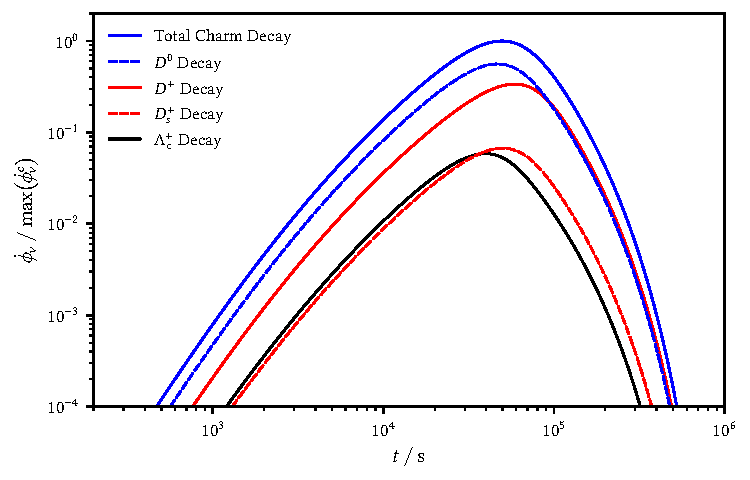
\includegraphics{../plots/build/magnetar_charm_decay_comparison_without.pdf}
	\caption[Magnetar $\nu \kern+0.5pt$ flux from $c$ decay excluding optical depth.]
			{Comparison of individual charmed hadron contributions to the total charm neutrino flux at
			 $E_\nu = \kern-0.5pt \qty{e9}{\giga\electronvolt}$ from a young magnetar, excluding the optical~depth
			 defined by \eqref{eqn:optical} as a modification. Properties of hadronic components in agreement with
			 Figure \ref{fig:magnetar-charm-comparison-with} are observed. Additionally, positions of maxima compatible
			 with lifetimes given in Section \ref{sub:charm} can be identified, as $\Lambda_{\kern+0.5pt c}^{\kern-0.5pt +}$
			 has the shortest decay timescale and therefore peaks first, while $D^+ \kern-0.5pt$ reaches its maximum after all other charmed
			 hadrons due to its longer lifetime.}
	\label{fig:magnetar-charm-comparison-without}
\end{figure}
